\begin{figure}[t]
	\centering
	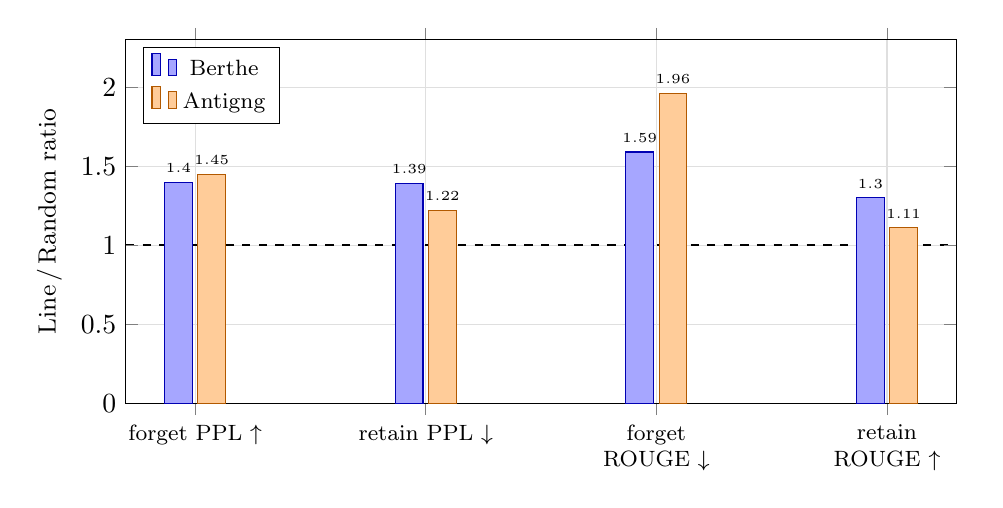
\begin{tikzpicture}
	\begin{axis}[
		ybar,
		bar width=10pt,
		width=\columnwidth,
		height=6.2cm,
		ylabel={Line\,/\,Random ratio},
		symbolic x coords={f\_PPL, r\_PPL, f\_ROUGE, r\_ROUGE},
		xtick=data,
		xticklabels={forget PPL $\uparrow$, retain PPL $\downarrow$, forget ROUGE $\downarrow$, retain ROUGE $\uparrow$},
		x tick label style={font=\footnotesize, align=center, text width=2cm},
		ymin=0, ymax=2.3,
		ytick={0, 0.5, 1.0, 1.5, 2.0},
		grid=major,
		grid style={gray!25},
		extra y ticks={1.0},
		extra y tick style={grid=major, grid style={black, thick, dashed}},
		extra y tick labels={},
		nodes near coords,
		nodes near coords style={font=\tiny, above},
		every node near coord/.append style={/pgf/number format/fixed, /pgf/number format/precision=2},
		every axis label/.style={font=\small},
		legend style={at={(0.02,0.98)}, anchor=north west, font=\footnotesize},
		clip=false,
	]
	\addplot[fill=blue!35, draw=blue!70!black] coordinates {
		(f\_PPL, 1.40)
		(r\_PPL, 1.39)
		(f\_ROUGE, 1.59)
		(r\_ROUGE, 1.30)
	};
	\addplot[fill=orange!40, draw=orange!70!black] coordinates {
		(f\_PPL, 1.45)
		(r\_PPL, 1.22)
		(f\_ROUGE, 1.96)
		(r\_ROUGE, 1.11)
	};
	\legend{Berthe, Antigng}
	\end{axis}
	\end{tikzpicture}
	\caption{NPO advantage of ob line-level forget sets over random baselines, per author. Each bar shows the ratio (line-level / random); metrics where lower is better are inverted so that $>$1 always indicates line-level outperforming random. Dashed line at 1.0 represents parity. Both authors dominate on all four metrics.}
	\label{fig:npo-advantage}
\end{figure}
